\chapter{ĐÊ XUẤT: NHẬN DẠNG NGÔN NGỮ KÝ HIỆU TỪ TỌA ĐỘ KHUNG XƯƠNG BẰNG MẠNG DNN}
\label{s:DNN}
Trong chương 3, thuật toán ước tính tư thế khung xương đã được trình bày chi tiết về lý thuyết và phương pháp xử lý áp dụng thuật toán. Ta thấy rằng phương pháp này hỗ trợ rất tốt cho việc ước tính nh anhtư thế khung xương trong xử lý thời gian thực. Trong chương 4 này, luận văn sẽ trình bày về đề xuất mô hình mạng DNN lấy đầu vào là toạ độ khung xương được ước tính và nhận dạng cử chỉ thời gian thực. Nội dụng chương trình bày cấu trúc mạng neural network đề xuất, cách thu thập và xử lý dữ liệu cũng như sơ đồ hoạt động chương trinh.
\section{Tổng quan}
Một hành động của con người được đánh giá, xem xét bằng một loạt các cử chỉ theo thời gian. Tuy nhiên, khi xem xét các hành động của con người nhằm tìm ra một cấu trúc nhất quán và có thể tạo thành mô hình thì gặp các vấn đề phức tạp sau:

$\bullet$ Nếu chỉ xem xét đường bao của con người, các phần cơ thể của con người quá gần nhau để có thể xác định được chính xác phần cơ thể cần thiết.

$\bullet$ Hình dạng của cử chỉ (đường bao con người, màu sắc các phần cơ thể), vị trí, loại và kiểu của cử chỉ rất phức tạp. Việc xem xét một mô hình có thể biểu diễn toàn bộ các hành động ngôn ngữ ký hiệu hầu như không thể xem xét nên trong phạm vi luận văn này chỉ xem xét đến việc một mô hình có thể biểu diễn 16 cử chỉ cần sự phối hợp cả hai tay và các cử chỉ tương đối khác nhau (\textbf{Xin chào, Tôi, thành phố, vui vẻ, ẵm em, Sài Gòn, Vĩnh Long, đi bộ, mùa màng, đói bụng, yêu, ăn, biểu quyết, đứng yên, hẹp, rộng}).

$\bullet$ Các hành động của con người có thể giống nhau, tuy nhiên nếu việc quan sát hoặc camera quan sát nằm ở vị trí khác nhau, hướng, độ cao,... đều ảnh hưởng đến khả năng nhận diện hành động của con người. Luận văn đã nêu được phương pháp để có thể phát triển cho việc xác định hành động của con người khi vị trí của camera thay đổi. Tuy nhiên việc kiểm chứng khả năng hoạt động ở các vị trí camera khác nhau sẽ được xem xét ở tương lai.

$\bullet$ Nếu một phần cơ thể bị che khuất bởi các vật thể thì việc xác định hành động của con người sẽ gặp khó khăn hơn rất nhiều so với trường hợp không bị che khuất, phạm vi luận văn không xem xét đến vấn đề này. Tuy nhiên đây là một điểm cần xem xét đến để có thể hoàn thiện hệ thống nhận diện cử chỉ trong tương lai.
\section{Thu thập dữ liệu}
Dữ liệu đầu vào là tọa độ của 18 khớp xương được detect từ mạng mobilenet. Các khớp xương được xuất ra từ mạng được đánh số thứ tự từ 0 tới 17. Các khớp xương cụ thể được thể hiện trong bảng \ref{table:joints} và trong hình \ref{fig:joints}.

\FloatBarrier
\begin{table}[h]
\caption{Các khớp xương được xuất ra từ mạng}
\label{table:joints}
\centering
\begin{center}
\begin{tabular}{|c|p{9cm}|} 
 \hline
Số thứ tự khớp xương  & Vị trí \\
 \hline
 0 & Mũi\\
 \hline 
 1 & Cổ\\
 \hline 
 2 & Vai phải\\
 \hline
 3 & Cùi chỏ phải \\
 \hline 
 4 & Cổ tay phải\\
 \hline
 5 & Vai trái\\
 \hline
 6 & Cùi chỏ trái\\
 \hline
 7 & Cổ tay trái\\
 \hline
 8 & Hông phải\\
 \hline
 9 & Đầu gối phải\\
 \hline
 10 & Cổ chân phải\\
 \hline
 11 & Hông trái\\
 \hline
 12 & Đầu gối trái\\
 \hline
 13 & Cổ chân trái\\
 \hline
 14 & Mắt phải\\
 \hline
 15 & Mắt trái\\
 \hline
 16 & Tai phải\\
 \hline
 17 & Tai trái\\
 \hline
\end{tabular}
\end{center}
\end{table}
\FloatBarrier

\FloatBarrier
\begin{figure}[htp]
\begin{center}
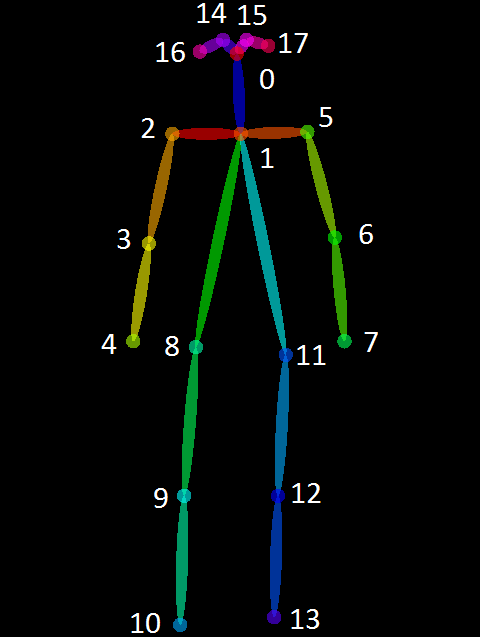
\includegraphics[scale=0.6]{chap4/c4_figs/joints_order.png}
\end{center}
\caption{Sơ đồ khớp xương xuất ra từ mạng mobilenet}
\label{fig:joints}
\end{figure}
\FloatBarrier

Ngôn ngữ ký hiệu với đặc trưng là phần trên cơ thể xuất hiện 
\section{Xử lý dữ liệu đầu vào}
\subsection{Loại bỏ các phần SJM dư thừa}

\subsection{Chuẩn hóa SJM để phân loại đặc trưng}
\FloatBarrier
\begin{figure}[htp]
\begin{center}
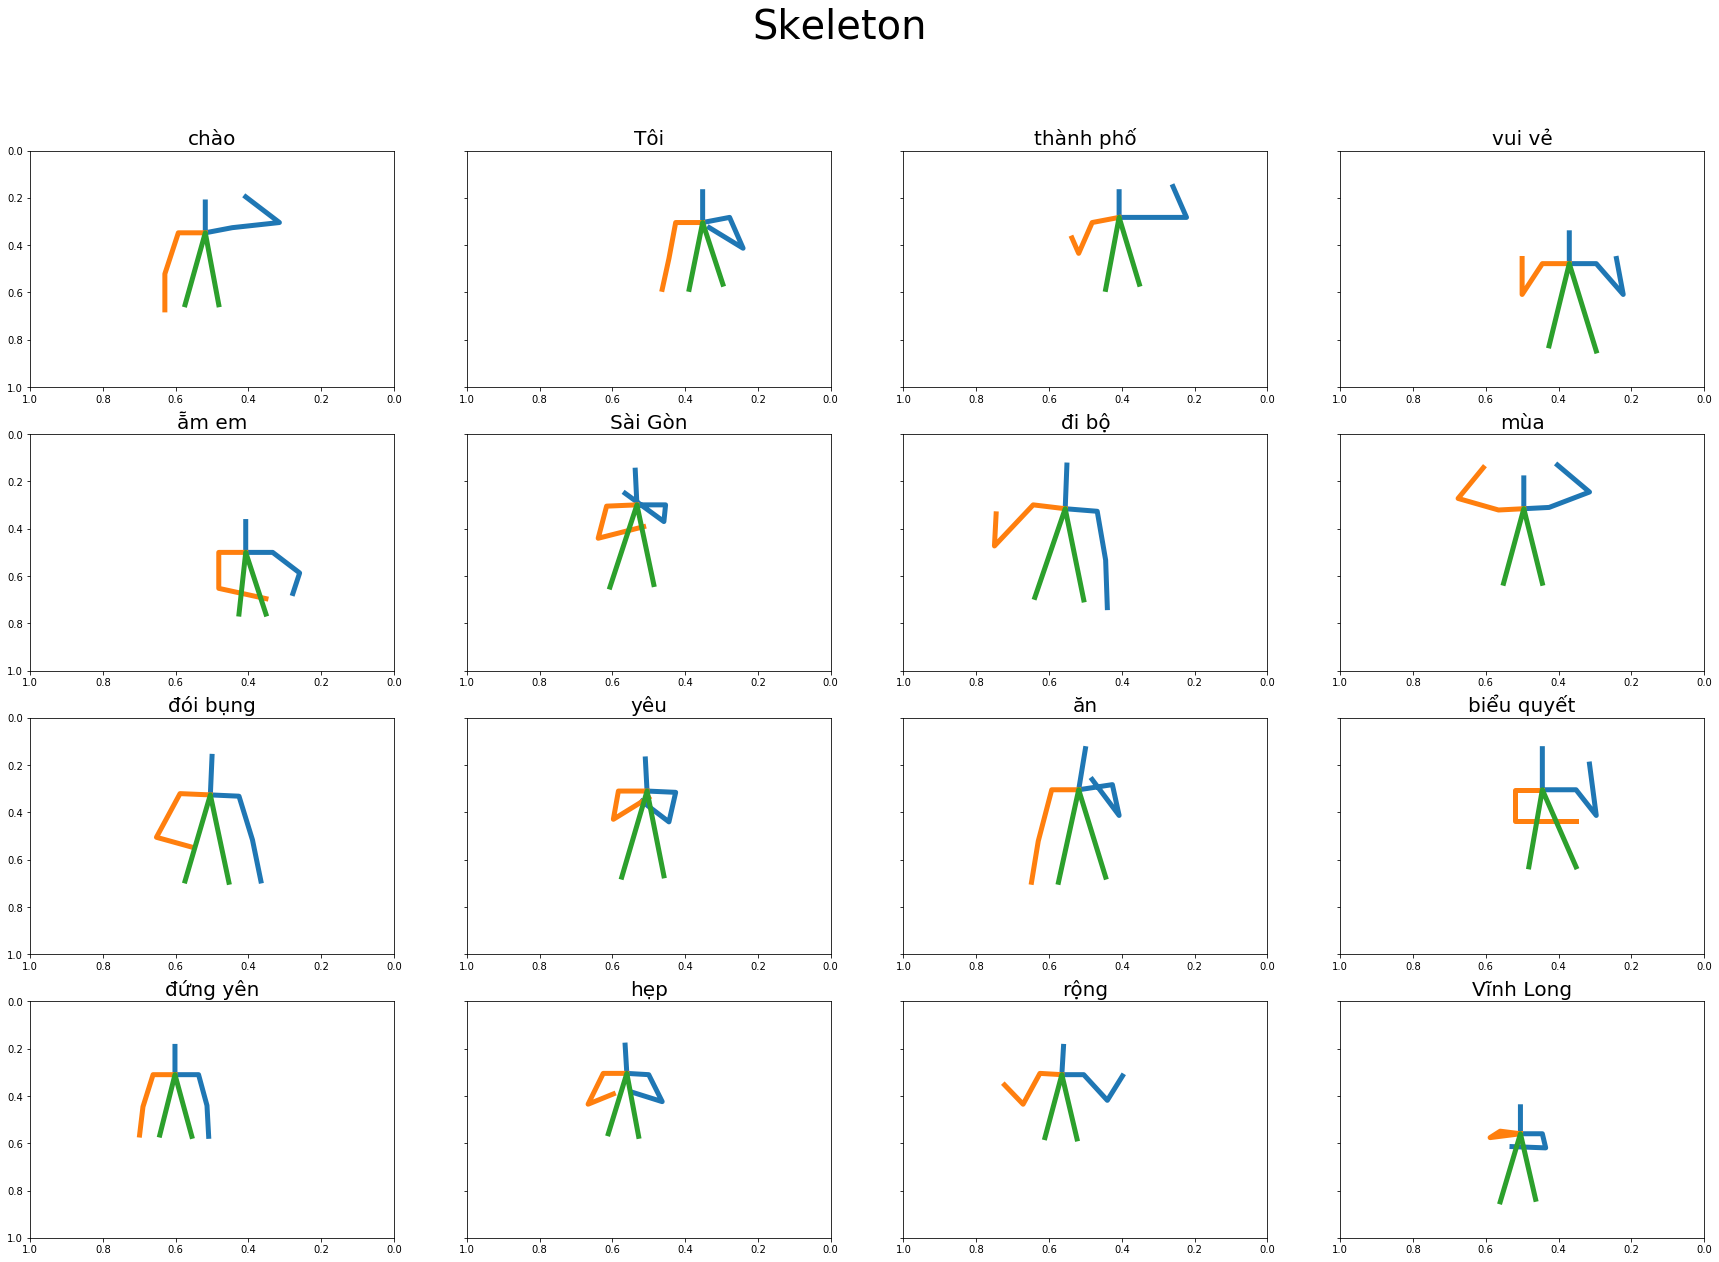
\includegraphics[scale=0.25]{chap4/c4_figs/datajoint.png}
\end{center}
\caption{Dữ liệu khớp xương sau khi đã loại bỏ hết các phần không cần thiết}
\label{fig:pipelineS}
\end{figure}
\FloatBarrier

\section{Cấu trúc mạng neural network đề xuất}

\section{Huấn luyện mạng}

\FloatBarrier
\begin{figure}[htp]
\begin{center}
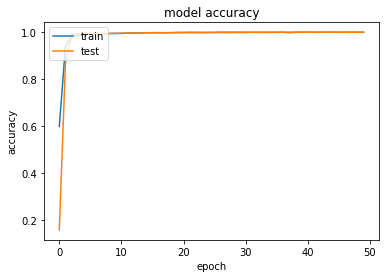
\includegraphics[scale=1]{chap4/c4_figs/train_val_acc.png}
\end{center}
\caption{Accurracy của tập train và validate}
\label{fig:pipelineS}
\end{figure}
\FloatBarrier

\FloatBarrier
\begin{figure}[htp]
\begin{center}
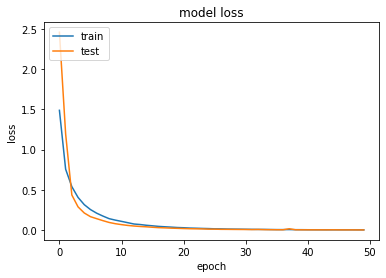
\includegraphics[scale=1]{chap4/c4_figs/train_val_l.png}
\end{center}
\caption{Loss của tập train và validate}
\label{fig:pipelineS}
\end{figure}
\FloatBarrier

\section{Kết quả}

\FloatBarrier
\begin{figure}[htp]
\begin{center}
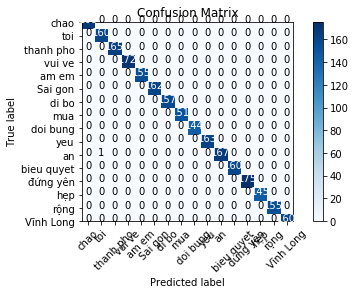
\includegraphics[scale=1]{chap4/c4_figs/confusion_matrix.png}
\end{center}
\caption{Confusion matrix của 16 lớp phân loại}
\label{fig:pipelineS}
\end{figure}
\FloatBarrier